This chapter outlines the foundational methodology employed throughout
the thesis. The research design adheres to a core set of principles,
fostering a continuous cycle of exploration, refinement, and
validation. The approach commences with the meticulous identification
of security challenges associated with resource protection within the
diverse domains of mobile and cloud applications. This initial phase
involves in-depth analysis of existing access control methods,
exposing limitations concerning their ability to provide fine-grained
control. Then, we identify threat models associated with the coarse
granularity. While there are inherent differences depending on the
specific context investigated, there is a common bottomline associated
with the exploitation of vulnerabilities, and how pervasive the use of
third-party software is in current mobile and cloud applications.
Indeed, running application components with broader permissions
translate into more attractive targets for attackers, as they can
reach a larger set of sensitive assets and escalate the attack.
Moreover, the common practice of using third-party software to speed
up development further exacerbates the problem, with developers
lagging behind with dependency updates and often disregarding the
trust implications of using external dependencies. % These problems
% are spread across the entire software industry and there are clear
% examples of them in mobile and cloud environments. For example, a
% common strategy to generate revenue from Android applications is to
% integrate Software Development Kits provided by advertising
% networks, however no guardrails exist to ensure the separation of
% this component from the core application. Another example is the
% extensive use of third-party services to enrich cloud applications
% with new functionalities. By running them alongside the application
% these services can capture sensitive information.

Informed by this analysis, the next phase involves the design of novel
access control mechanisms that specifically target fine-grained
enforcement. The design process encompasses the meticulous evaluation
of enforcement models, creation of security policies, and careful
consideration of integration strategies for seamless operation within
the established system architectures. Despite the differences between
mobile and cloud architectures, when we consider Android (i.e., the
mobile operating system holding 69.94\% of the market
share~\cite{android-os-marker-share}), Figure~\ref{fig:methodology}
shows they share a common foundation: the Linux kernel. By leveraging
the built-in security features of the Linux kernel (e.g., seccomp,
eBPF, Landlock, SELinux), this thesis proposes an efficient approach
to establishing fine-grained access control across mobile and cloud
environments. This approach not only addresses specific challenges in
each domain but also demonstrates the versatility and potential of the
Linux kernel as a foundation for diverse application domains.

\begin{figure}[t]
    \centering
    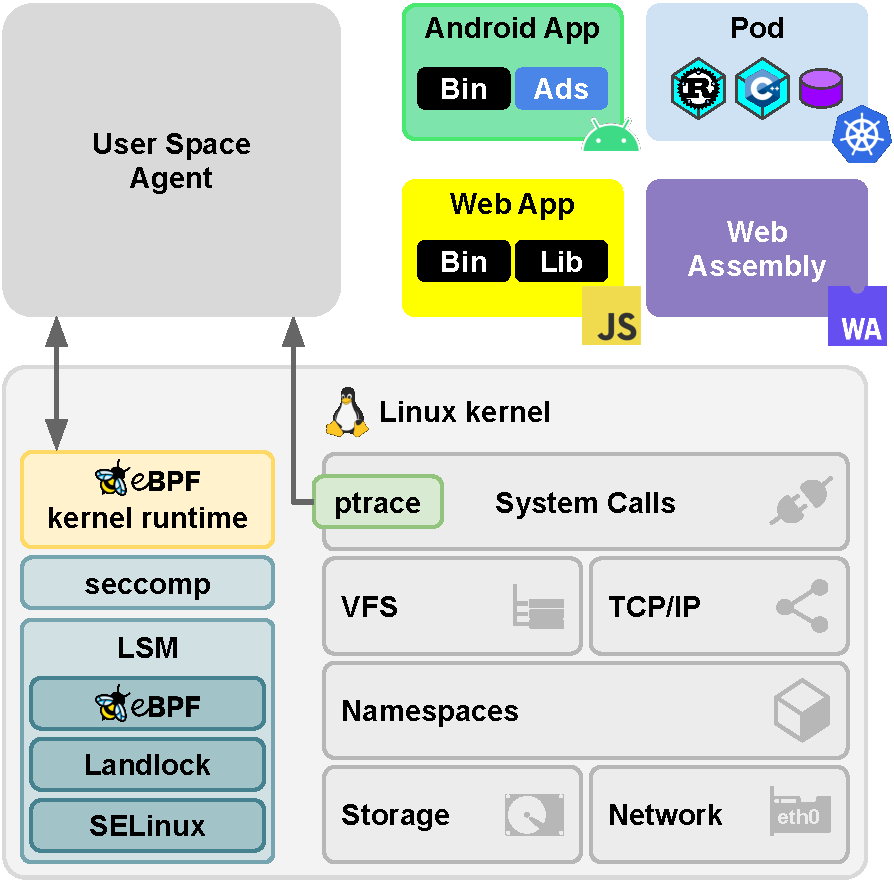
\includegraphics[width=0.8\columnwidth]{
        chapters/methodology/fig/methodology
    }
    \caption[High-level overview of the research methodology]{
        High-level overview of the methodology for integrating the use
        of fine-grained access control technologies in mobile and
        cloud applications
    }
    \label{fig:methodology}
\end{figure}

Following the design of the solution, the next step involves its
implementation utilizing programming languages, frameworks, and tools
specifically chosen for their suitability within the targeted
environments. Then, extensive evaluation follows, utilizing a
combination of security testing and performance measurement
techniques. Security testing meticulously evaluates the capability of
the solution to enforce security policies and prevent unauthorized
resource access. This consists of reproducing common vulnerabilities
classes and public proofs of concept to appraise the ability to
mitigate attacks. Performance evaluation examines the overheads
introduced by the solution, assessing metrics such as execution time
and throughput. The findings serve as the cornerstone for the
iterative refinement and improvement of the proposed solutions. This
cyclical process addresses any identified shortcomings, optimizes
efficiency, and ultimately ensures the robustness of the fine-grained
access control mechanisms. Prototype implementations are open-source
to promote reproducibility of our experimental results and ease of
integration with existing systems.

While the specific technical details and implementation nuances
vary between mobile and cloud environments due to their inherent
differences, the overarching methodological framework described in
this chapter provides a concise summary of the research approach
adopted, but also highlights the potential of leveraging shared
underlying features to address security challenges across diverse
technological domains.
